\chapter{Experiments and Evaluation}
\label{cha:Experiments and Evaluation}
%\lipsum \autocite{DBLP:books/sp/HarderR01}

\section{Experiments}

The proposed experiments will build on the scenarios from \autocite{maximilian}. The experiments included three parcours with different difficulty levels \ref*{fig:3tracks} and conducted 3 different experiments with each trained agent. The first experiment was under optimal conditions with minimal changes from the simulation environment. The second experiment was conducted under different lighting settings. The third one changed the motor power of the agent's two front wheels.

The experiment with minimal changes and changed lighting settings will be used to evaluate the agent developed in this thesis. Using the same experiments allows for an easy comparison to the previous research. The experiment with varying motor power will be omitted since it is not related to the research goals of this thesis.

The experiments under minimal changes will be used to judge if the agent is able to reliably solve all parcours and hence answer the first research question. Agents with and without memory capabilities will be compared to investigate the contributions of the memory mechanism.

The experiment with varying lighting settings will be used to evaluate the agent's robustness towards changing light conditions and hence answer the second research question. Comparing the results of the agents with differently sized CNNs will provide insights into the required size and complexity of the CNNs. This will be used to judge if the agents can be transferred to real-life NVIDIA JetBots at the Scads.AI research facility.

The results of both experiments will be compared to the previous work's results to see if the CNN approach outperformed the engineered preprocessing pipeline.


\begin{figure}
    \centering
    \subfigure[Easy]{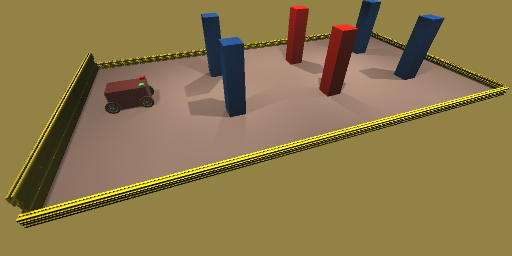
\includegraphics[width=0.5\textwidth]{Bilder/evaluation_easy.png}}\qquad
    \subfigure[Medium]{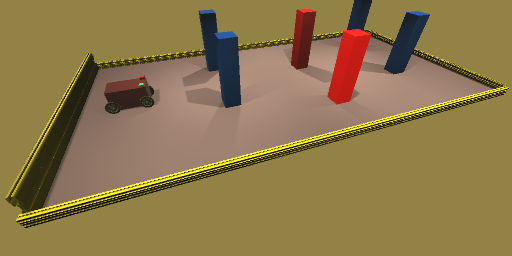
\includegraphics[width=0.5\textwidth]{Bilder/evaluation_medium.png}}\qquad
    \subfigure[Hard]{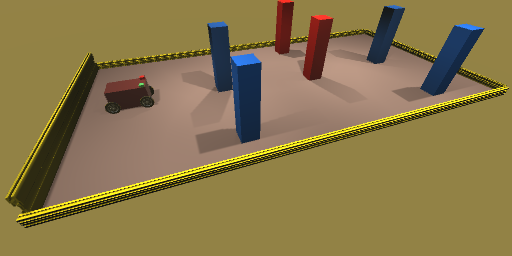
\includegraphics[width=0.5\textwidth]{Bilder/evaluation_hard.png}}\qquad
    \caption{Evaluation Tracks of different difficulties}
    \label{fig:3tracks}
\end{figure}

\section{Evaluation}

During the training and the final experiments, the agents are evaluated using the success rate, the average time needed to complete the map and the collision rate. The success rate is the percentage of episodes in which the agent successfully completed the map. These metrics were already used by \autocite{maximilian} and measure the most important properties of the agent's behaviour.

There will be additional metrics monitored during the training process to identify weak-points of the agent and erroneous behaviour. Monitoring the training process can provide insights into the agent's behaviour and help with choosing appropriate hyperparameters.
These metrics could be the average cumulative reward, the average number of passed goals, the average distance travelled, the average amount of collisions, the average game duration and the average speed of the agent.


% kann ich die Experimente mit varying motor power weglassen?
% die Experimente stehen nicht so stark im Zusammenhang mit den beiden Research goals
% ja